\documentclass[a4paper]{article}
\usepackage[a4paper,margin=1in,landscape]{geometry}
\usepackage[utf8]{inputenc}
\usepackage[T1]{fontenc}
\usepackage{longtable}
\usepackage[table,svgnames]{xcolor}
\usepackage{colortbl}
\usepackage{pgfplots}
\pgfplotsset{width=10cm,compat=1.14}
\usepgfplotslibrary{dateplot}
\usetikzlibrary{plotmarks}
\usepackage{booktabs}
\usepackage{array}
\usepackage{eurosym}
\usepackage{forest}
\usepackage{listings}
\usepackage{multicol}
\usepackage{fancyhdr}
\pagestyle{fancy}
\lfoot{Section \leftmark}
\cfoot{}
\rfoot{\thepage}
\rhead{Generated: \today}
\chead{}
\lhead{Scheduling Report}
\usepackage{hyperref}
\title{Scheduling Report}
\author{L. O'Toole and H. Simonis}
\date{Report Generated on \today}

\begin{document}
\maketitle
\definecolor{wipcolor}{RGB}{128,128,128}
\definecolor{downcolor}{RGB}{255,0,0}
\definecolor{latecolor}{RGB}{255,0,0}
\definecolor{makespancolor}{RGB}{255,0,0}
\definecolor{resourcecolor}{RGB}{0,0,255}
\definecolor{jobcolor}{RGB}{0,255,0}
\definecolor{stagecolor0}{RGB}{240,163,255}
\definecolor{stagecolor1}{RGB}{0,117,220}
\definecolor{stagecolor2}{RGB}{153,63,0}
\definecolor{stagecolor3}{RGB}{76,0,92}
\definecolor{stagecolor4}{RGB}{25,25,25}
\definecolor{stagecolor5}{RGB}{0,92,49}
\definecolor{stagecolor6}{RGB}{43,206,72}
\definecolor{stagecolor7}{RGB}{255,204,153}
\section{Introduction}

\begin{table}[htbp]
\caption{Problem}
\centering
\begin{tabular}{llrrrrrrrr} \toprule
Name &Label &\shortstack{Timepoints\\as\\Date} &\shortstack{Nr\\Products} &\shortstack{Nr\\Process} &\shortstack{Nr\\Disjunctive\\Resources} &\shortstack{Nr\\Cumulative\\Resources} &\shortstack{Nr\\Orders} &\shortstack{Nr\\Jobs} &\shortstack{Nr\\Tasks} \\ \midrule
Generated&JSON Doc&true&1&1&1&1&1&1&2\\ 
\bottomrule
\end{tabular}
\end{table}

\section{Solution}

\begin{table}[htbp]
\caption{Relaxation of Constraints}
\centering
\begin{tabular}{llrrrrrrr} \toprule
Name &Label &\shortstack{Enforce\\Release\\Date} &\shortstack{Enforce\\Due\\Date} &\shortstack{Enforce\\Cumulative} &\shortstack{Enforce\\WiP} &\shortstack{Enforce\\Downtime} &\shortstack{Nr\\Threads} &\shortstack{Timeout\\(s)} \\ \midrule
Sol1&&\cellcolor{white}true&\cellcolor{red!30}false&\cellcolor{white}true&\cellcolor{white}true&\cellcolor{white}true&2&30\\ 
\bottomrule
\end{tabular}
\end{table}

\begin{table}[htbp]
\caption{Solutions (Total 1)}
\centering
\begin{tabular}{lllrrrrrrrrrrrlr} \toprule
Name &\shortstack{Solver\\Status} &\shortstack{Objective\\Type} &\shortstack{Objective\\Value} &Bound &Gap &Makespan &Flowtime &\shortstack{Total\\Lateness} &\shortstack{Max\\Lateness} &\shortstack{Nr\\Late} &\shortstack{Total\\Earliness} &\shortstack{Max\\Earliness} &\shortstack{Nr\\Early} &\shortstack{Model\\Type} &\shortstack{Time\\(s)} \\ \midrule
Sol1&Optimal&Makespan&163&163.00& 0.00&163&163&0&0&0&1,832&1,832&\cellcolor{red!40}1&CPO& 0.09\\ 
\bottomrule
\end{tabular}
\end{table}

\begin{figure}[htbp]
\caption{Cost of Intermediate Solutions}
\centering
\begin{tikzpicture}
\begin{axis}[xlabel=Time (s),ylabel=Cost,,width=23cm,height=12cm]
\addplot+[] coordinates {
    (0.0100000,163.000)
};
\end{axis}
\end{tikzpicture}

\end{figure}

\begin{figure}[htbp]
\caption{Machine Gantt for Solution Sol1}
\label{resourceGantt1}
\centering
\begin{tikzpicture}[xscale=1.000000,yscale=1.000000]
\draw[draw=black!20] (0.000000,1.000000) -- (0.000000,-0.100000);
\node[below] at (0.000000,-0.100000) {0};
\draw[draw=black!20] (2.822086,1.000000) -- (2.822086,-0.100000);
\node[below] at (2.822086,-0.100000) {20};
\draw[draw=black!20] (5.644172,1.000000) -- (5.644172,-0.100000);
\node[below] at (5.644172,-0.100000) {40};
\draw[draw=black!20] (8.466258,1.000000) -- (8.466258,-0.100000);
\node[below] at (8.466258,-0.100000) {60};
\draw[draw=black!20] (11.288344,1.000000) -- (11.288344,-0.100000);
\node[below] at (11.288344,-0.100000) {80};
\draw[draw=black!20] (14.110429,1.000000) -- (14.110429,-0.100000);
\node[below] at (14.110429,-0.100000) {100};
\draw[draw=black!20] (16.932515,1.000000) -- (16.932515,-0.100000);
\node[below] at (16.932515,-0.100000) {120};
\draw[draw=black!20] (19.754601,1.000000) -- (19.754601,-0.100000);
\node[below] at (19.754601,-0.100000) {140};
\draw[draw=black!20] (22.576687,1.000000) -- (22.576687,-0.100000);
\node[below] at (22.576687,-0.100000) {160};
\draw[draw=black!20] (0.000000,1.000000) -- (0.000000,-0.050000);
\draw[draw=black!20] (1.411043,1.000000) -- (1.411043,-0.050000);
\draw[draw=black!20] (2.822086,1.000000) -- (2.822086,-0.050000);
\draw[draw=black!20] (4.233129,1.000000) -- (4.233129,-0.050000);
\draw[draw=black!20] (5.644172,1.000000) -- (5.644172,-0.050000);
\draw[draw=black!20] (7.055215,1.000000) -- (7.055215,-0.050000);
\draw[draw=black!20] (8.466258,1.000000) -- (8.466258,-0.050000);
\draw[draw=black!20] (9.877301,1.000000) -- (9.877301,-0.050000);
\draw[draw=black!20] (11.288344,1.000000) -- (11.288344,-0.050000);
\draw[draw=black!20] (12.699387,1.000000) -- (12.699387,-0.050000);
\draw[draw=black!20] (14.110429,1.000000) -- (14.110429,-0.050000);
\draw[draw=black!20] (15.521472,1.000000) -- (15.521472,-0.050000);
\draw[draw=black!20] (16.932515,1.000000) -- (16.932515,-0.050000);
\draw[draw=black!20] (18.343558,1.000000) -- (18.343558,-0.050000);
\draw[draw=black!20] (19.754601,1.000000) -- (19.754601,-0.050000);
\draw[draw=black!20] (21.165644,1.000000) -- (21.165644,-0.050000);
\draw[draw=black!20] (22.576687,1.000000) -- (22.576687,-0.050000);
\draw[draw=black!20] (23.987730,1.000000) -- (23.987730,-0.050000);
\node[draw=black,fill=resourcecolor!10,font=\scriptsize,minimum height=0.800000cm,above left] (DR0) at (0,0.000000) {DR0};
\draw[draw=black,fill=stagecolor0!10] (6.067485,0.000000) rectangle node {} (14.533742,0.800000);
\draw[draw=black,fill=stagecolor1!10] (14.533742,0.000000) rectangle node {} (23.000000,0.800000);
\draw[draw=black,fill=wipcolor!40] (0.000000,0.000000) rectangle node {} (6.067485,0.800000);
\draw[draw=makespancolor,thick] (23.000000,1.000000) -- (23.000000,0.000000);
\node[above left,font=\scriptsize] () at (23.000000,1.000000) {Cmax: 163};
\node[left,] () at (3.000000,-1.000000) {WiP};
\node[right,draw=black,fill=wipcolor!40,font=\scriptsize] () at (3.000000,-1.000000) {};
\node[left,] () at (5.000000,-1.000000) {Stage0};
\node[right,draw=black,fill=stagecolor0!10,font=\scriptsize] () at (5.000000,-1.000000) {};
\node[left,] () at (7.000000,-1.000000) {Stage1};
\node[right,draw=black,fill=stagecolor1!10,font=\scriptsize] () at (7.000000,-1.000000) {};
\node[left,] () at (9.000000,-1.000000) {Late};
\node[right,draw=latecolor,font=\scriptsize] () at (9.000000,-1.000000) {};
\end{tikzpicture}
\end{figure}
\begin{figure}[htbp]
\caption{Job Gantt for Solution Sol1}
\label{jobGantt1}
\centering
\begin{tikzpicture}[xscale=1.000000,yscale=1.000000]
\draw[draw=black!20] (1.341667,1.000000) -- (1.341667,-0.100000);
\node[below] at (1.341667,-0.100000) {50};
\draw[draw=black!20] (3.258333,1.000000) -- (3.258333,-0.100000);
\node[below] at (3.258333,-0.100000) {60};
\draw[draw=black!20] (5.175000,1.000000) -- (5.175000,-0.100000);
\node[below] at (5.175000,-0.100000) {70};
\draw[draw=black!20] (7.091667,1.000000) -- (7.091667,-0.100000);
\node[below] at (7.091667,-0.100000) {80};
\draw[draw=black!20] (9.008333,1.000000) -- (9.008333,-0.100000);
\node[below] at (9.008333,-0.100000) {90};
\draw[draw=black!20] (10.925000,1.000000) -- (10.925000,-0.100000);
\node[below] at (10.925000,-0.100000) {100};
\draw[draw=black!20] (12.841667,1.000000) -- (12.841667,-0.100000);
\node[below] at (12.841667,-0.100000) {110};
\draw[draw=black!20] (14.758333,1.000000) -- (14.758333,-0.100000);
\node[below] at (14.758333,-0.100000) {120};
\draw[draw=black!20] (16.675000,1.000000) -- (16.675000,-0.100000);
\node[below] at (16.675000,-0.100000) {130};
\draw[draw=black!20] (18.591667,1.000000) -- (18.591667,-0.100000);
\node[below] at (18.591667,-0.100000) {140};
\draw[draw=black!20] (20.508333,1.000000) -- (20.508333,-0.100000);
\node[below] at (20.508333,-0.100000) {150};
\draw[draw=black!20] (22.425000,1.000000) -- (22.425000,-0.100000);
\node[below] at (22.425000,-0.100000) {160};
\draw[draw=black!20] (0.383333,1.000000) -- (0.383333,-0.050000);
\draw[draw=black!20] (1.341667,1.000000) -- (1.341667,-0.050000);
\draw[draw=black!20] (2.300000,1.000000) -- (2.300000,-0.050000);
\draw[draw=black!20] (3.258333,1.000000) -- (3.258333,-0.050000);
\draw[draw=black!20] (4.216667,1.000000) -- (4.216667,-0.050000);
\draw[draw=black!20] (5.175000,1.000000) -- (5.175000,-0.050000);
\draw[draw=black!20] (6.133333,1.000000) -- (6.133333,-0.050000);
\draw[draw=black!20] (7.091667,1.000000) -- (7.091667,-0.050000);
\draw[draw=black!20] (8.050000,1.000000) -- (8.050000,-0.050000);
\draw[draw=black!20] (9.008333,1.000000) -- (9.008333,-0.050000);
\draw[draw=black!20] (9.966667,1.000000) -- (9.966667,-0.050000);
\draw[draw=black!20] (10.925000,1.000000) -- (10.925000,-0.050000);
\draw[draw=black!20] (11.883333,1.000000) -- (11.883333,-0.050000);
\draw[draw=black!20] (12.841667,1.000000) -- (12.841667,-0.050000);
\draw[draw=black!20] (13.800000,1.000000) -- (13.800000,-0.050000);
\draw[draw=black!20] (14.758333,1.000000) -- (14.758333,-0.050000);
\draw[draw=black!20] (15.716667,1.000000) -- (15.716667,-0.050000);
\draw[draw=black!20] (16.675000,1.000000) -- (16.675000,-0.050000);
\draw[draw=black!20] (17.633333,1.000000) -- (17.633333,-0.050000);
\draw[draw=black!20] (18.591667,1.000000) -- (18.591667,-0.050000);
\draw[draw=black!20] (19.550000,1.000000) -- (19.550000,-0.050000);
\draw[draw=black!20] (20.508333,1.000000) -- (20.508333,-0.050000);
\draw[draw=black!20] (21.466667,1.000000) -- (21.466667,-0.050000);
\draw[draw=black!20] (22.425000,1.000000) -- (22.425000,-0.050000);
\draw[draw=black!20] (23.383333,1.000000) -- (23.383333,-0.050000);
\node[draw=black,fill=jobcolor!10,font=\scriptsize,minimum height=0.800000cm,above left] (J0) at (0,0.000000) {J0};
\draw[draw=black,fill=stagecolor0!10] (0.000000,0.000000) rectangle node {} (11.500000,0.800000);
\draw[draw=black,fill=stagecolor1!10] (11.500000,0.000000) rectangle node {} (23.000000,0.800000);
\draw[draw=makespancolor,thick] (23.000000,1.000000) -- (23.000000,0.000000);
\node[above left,font=\scriptsize] () at (23.000000,1.000000) {Cmax: 163};
\node[left,] () at (3.000000,-1.000000) {Stage0};
\node[right,draw=black,fill=stagecolor0!10,font=\scriptsize] () at (3.000000,-1.000000) {};
\node[left,] () at (5.000000,-1.000000) {Stage1};
\node[right,draw=black,fill=stagecolor1!10,font=\scriptsize] () at (5.000000,-1.000000) {};
\node[left,] () at (7.000000,-1.000000) {Late};
\node[right,draw=latecolor,font=\scriptsize] () at (7.000000,-1.000000) {};
\end{tikzpicture}
\end{figure}
\begin{figure}[htbp]
\caption{Resource Utilization for Solution Sol1}
\centering
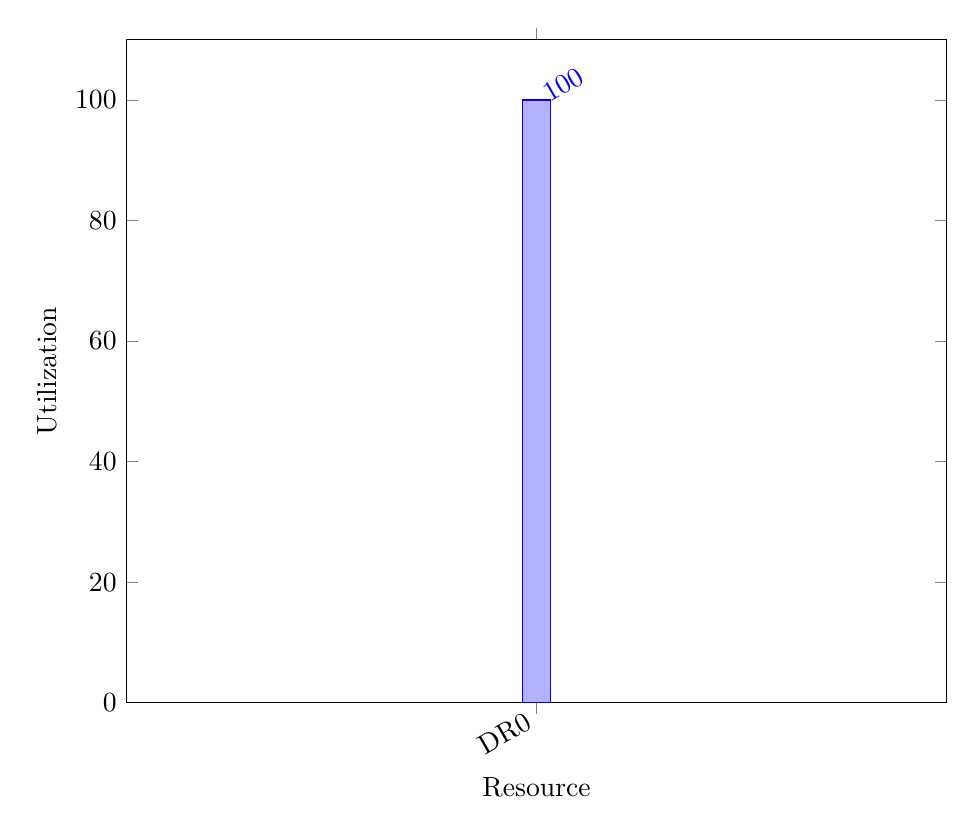
\begin{tikzpicture}
\begin{axis}[xlabel=Resource,ylabel=Utilization,ymin=0,
width=12cm,height=10cm,ybar,
symbolic x coords={DR0},
    xtick=data,nodes near coords, nodes near coords align={rotate=30),anchor=west},x tick label style={rotate=30),anchor=east}]
\addplot+[] coordinates {
(DR0,100.000000)
};
\end{axis}
\end{tikzpicture}

\end{figure}

\begin{figure}[htbp]
\caption{Cumulative Resource Use CR0}
\centering
\begin{tikzpicture}
\begin{axis}[xlabel=Time,ylabel=Resource Use,enlarge x limits=0.01,no markers,,legend pos=outer north east,xmin=0,xmax=163,width=21cm,height=12cm]
\addplot+ [const plot] coordinates {
    (0,5)
    (163,0)
    (163,0)
};
\addlegendentry{Capacity}
\addplot+ [const plot] coordinates {
    (0,0)
    (43,1)
    (163,0)
    (163,0)
};
\addlegendentry{Demand}
\end{axis}
\end{tikzpicture}

\end{figure}

\begin{figure}[htbp]
\caption{Earliness/Lateness Over Time}
\centering
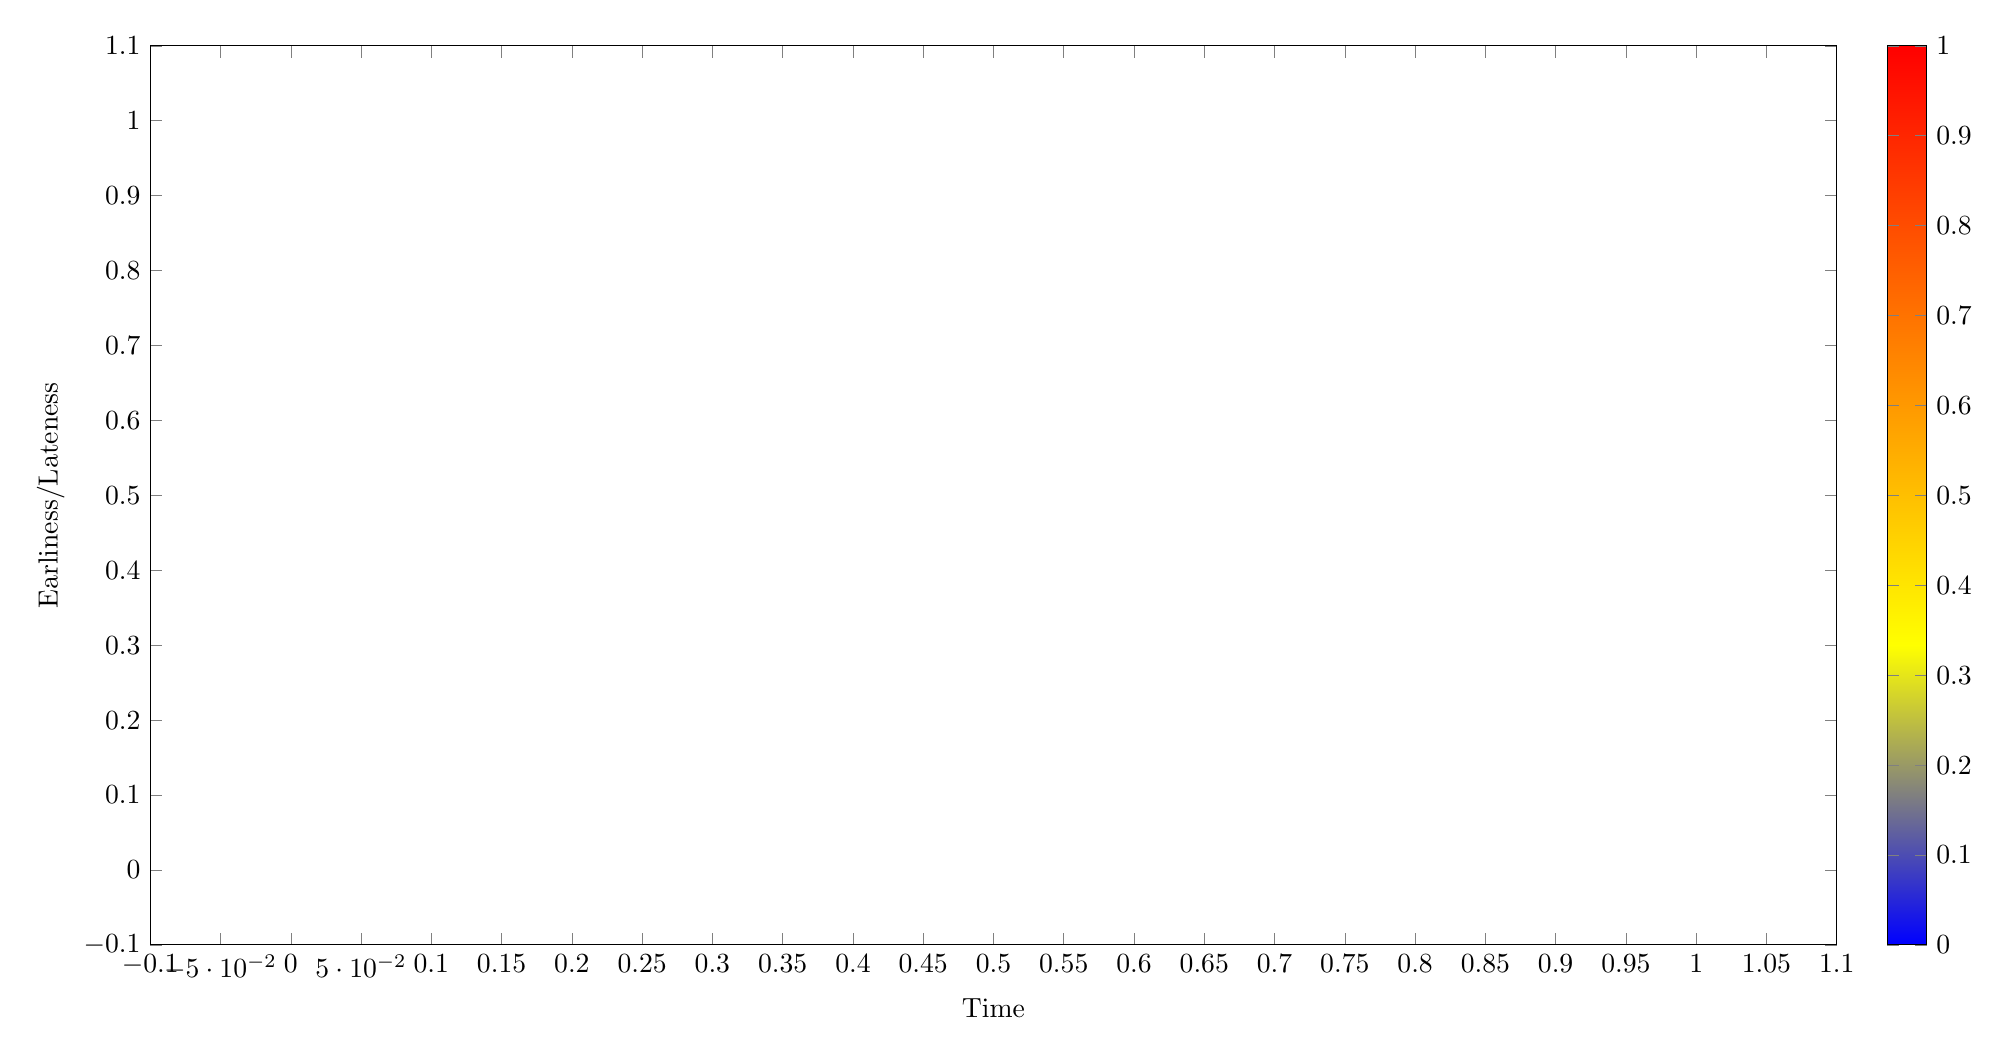
\begin{tikzpicture}
\begin{axis}[xlabel=Time,ylabel=Earliness/Lateness,,width=23cm,height=13cm,colorbar]
\draw[draw=red] (163.000000,\pgfkeysvalueof{/pgfplots/ymin}) -- node[right] {163} (163.000000,\pgfkeysvalueof{/pgfplots/ymax});

\draw[draw=red] (\pgfkeysvalueof{/pgfplots/xmin},0.000000) -- node[above] {Max Delay: 0} (\pgfkeysvalueof{/pgfplots/xmax},0.000000);

\draw[draw=blue] (\pgfkeysvalueof{/pgfplots/xmin},-1832.000000) -- node[above] {Max Early: 1,832} (\pgfkeysvalueof{/pgfplots/xmax},-1832.000000);

\draw[draw=black] (\pgfkeysvalueof{/pgfplots/xmin},0.000000) -- node[above] {On-time} (\pgfkeysvalueof{/pgfplots/xmax},0.000000);

\end{axis}
\end{tikzpicture}

\end{figure}

\end{document}
